\chapter{État de l'art}

\section{Introduction}

\lettrine{L}{a configuration} des composantes logicielles impose un coût majeur
dans l'administration d'un système. Des erreurs de configuration peuvent se
traduire par des vulnérabilités en termes de sécurité, de sévères perturbations
dans le fonctionnement de la brique logicielle, ou purement et simplement
provoquer un déni de service. La prise en considération du contexte pourrait
permettre une abstraction partielle ou complète de cette couche très technique
et extrêmement pénible à configurer.

Un système sensible au contexte doit être capable de mimer la capacité humaine à
reconnaître et exploiter l'information implicitement présente dans
l'environnement. Cela implique une configuration dynamique de chacune des
composantes de l'architecture, de manière à pouvoir ajuster leur comportement
respectif en fonction de la situation. Identifier l'activité humaine est un
défi certain, il est essentiel que les applications opèrent en transmettant
l'information appropriée au bon endroit et au bon moment par inférence de
l'intention des utilisateurs. L'informatique sensible au contexte est un
paradigme dans lequel les applications peuvent découvrir et tirer profit d'
informations de circonstance telles que la position actuelle, l'heure de la
journée, les personnes et périphériques dans l'environnement et leurs activités.

Dans ce mémoire, nous aborderons dans un premier temps les principes communs à
chacune des solutions existantes. Ces concepts seront résumés à l'aide d'un
framework conceptuel dérivé par couches. Nous présenterons un certaine variété
d'infrastructures et d'intergiciels reconnus pour faciliter la configuration
d'applications et de services basés sur le contexte. Dans un second temps, nous
proposerons un modèle d'abstraction des informations de contexte basé sur les
ontologies. Ce modèle met en corrélation des concepts tels que le consensus de
raft et la théorie de la promesse pour aboutir à un système distribué permettant
la coordination d'informations de contexte. Enfin, nous apporterons une preuve de
concept par une implémentation du modèle en langage Python.

\section{Contexte}

De nombreux débats ont eu lieu et continuent de voir le jour sur le sens du
contexte et de l'informatique sensible au contexte. Alors que la plupart des
gens comprennent de manière tacite ce qu'est le contexte, ils le trouve par
ailleurs particulièrement difficile à élucider.

{%\begin{figure}[H]
    \centering
    \begin{tabular}{l}
        ``... toute information pouvant être utilisée pour caractériser la
        situation d'une entité.\\ 
        Une entité peut être une personne, un lieu ou un objet considéré
        pertinent dans l'interaction \\ 
        entre un utilisateur et une application, notamment l'utilisateur et
        l'application eux même.``
        \cite{abowd_baltzer_1997} \\
        %\em \footnotesize Gregory D. Abowd, Christopher G. Atkeson, Jason Hong,
        %Sue Long, Rob Kooper, and Mike \\
        %\em \footnotesize Pinkerton. Cyberguide: a mobile context-aware tour
        %guide. Wireless Networks, 3(5):421–433, Octobre 1997. 
    \end{tabular}
    %\caption{Le contexte défini par Abowd et. al. (1997)}
    %\label{fig:quote}
}%\end{figure}

Cette définition rend la tâche plus facile à un développeur d'application pour
énumérer le contexte dans un scénario d'application donné. Si un fragment
d'information peut être utilisé pour caractériser la situation d'un participant
dans une quelconque interaction, alors cette information appartient au contexte.

\section{Vue d'ensemble sur le contexte}

{%\begin{figure}[H]
    \centering
    \begin{tabular}{l}
        ``Le contexte est efficace, seulement lorsqu'il est partagé.``
        \cite{winograd_architectures_2001} \\
        %\em \footnotesize Terry Winograd. Architectures for Context. \\
        %\em \footnotesize Human-Computer Interaction, 16(2):401–419,
        % Décembre 2001. \\
    \end{tabular}
    %\caption{Winograd à propos du contexte (2001)}
    %\label{fig:quote}
}%\end{figure}

Pour s'assurer que le contexte soit partagé, il doit d'abord être recueilli et
rigoureusement traité. Cela implique qu'un système sensible au contexte doit
être en mesure de comprendre ce qu'est le contexte avant d'aller à la recherche
de ces informations et de pouvoir les catégoriser.

\subsection{Classes de contexte}

Schilit et al. proposent la classification suivante des informations de
contexte:

\begin{itemize}
    \item \textbf{Contexte informatique} - Connectivité réseau, bande passante,
        et ressources à proximité telles que des imprimantes, des affichages ou
        des postes de travail.
    \item \textbf{Contexte utilisateur} - Le profil utilisateur, sa situation
        géographique, sa situation sociale actuelle et les individus qui
        l'entourent.
    \item \textbf{Contexte physique} - L'éclairage, le niveau de bruit, les
        condition de circulation ou la température.
\end{itemize}

Chacune de ces catégories contiennent une richesse d'informations pertinentes
pour le système sensible au contexte. Elle ne peuvent cependant pas être
traitées de manière isolée pour pouvoir en extraire le meilleur. L'intention du
système sensible au contexte est de rassembler et de fusionner ces informations
pour aboutir à une vue d'ensemble de la situation. Une fois le contexte mis en
tampon ou en base, le système doit alors filtrer les informations pertinentes
pour l'utilisateur, dans le moment présent.

Les informations de contexte peuvent alternativement être subdivisées en 2
catégories bien distinctes: contexte virtuel ou physique.

\subsubsection{Contexte virtuel}

Le contexte virtuel inclut la version du système d'exploitation, les
possibilités d'interface, la technologie en charge de l'accomplissement des
communications, les emails envoyés et reçus, et les documents édités. Autrement
dit, il s'agit là de tous les faits non tangibles. Pierre Lévy donne une
définition intéressante du contexte virtuel à travers une question assez
philosophique :

{%\begin{figure}[H]
    \centering
    \begin{tabular}{l}
        ``Pourquoi la consommation d'une information n'est-elle pas destructive
        \\ et sa détention n'est-elle pas exclusive ? \\ 
        Parce que l'information est virtuelle``
        \cite{levy_quest_2010} \\
        %\em \footnotesize Pierre Lévy. Qu'est ce que le virtuel ?\\
        %\em \footnotesize La découverte, 56/159, Juillet 2010. \\
    \end{tabular}
    %\caption{Le contexte virtuel par Pierre Lévy (2010)}
    %\label{fig:quote}
}%\end{figure}

\subsubsection{Contexte physique}

Les contexte physique d'un autre coté peut se traduire par la présence d'une
autre entité, qu'elle soit utilisateur ou périphérique, la proximité d'une
imprimante en particulier, une indication que l'utilisateur est debout, en train
de marcher ou assis ou même les conditions météorologiques actuelles. En d'autres
termes, le contexte physique peut être défini comme toute donnée acquérable par
le biais d'un capteur.

\subsubsection{Contexte historique}

Les contextes mémorisés au cours d'un certain laps de temps. Cette information
est considérée très utile, mais n'est que très rarement utilisée, sauf peut-être
par les applications mobiles. Le système doit être en mesure d'estimer les
informations valant la peine d'être conservées. Cette évaluation est
excessivement coûteuse et nécessite donc des algorithmes très performants.

\subsection{Les caractéristiques des informations de contexte}

Les chercheurs l'université de Queensland ont classifié quatre caractéristiques
majeures : \cite{catharina_context_2002}

\begin{enumerate}
    \item \textbf{Les informations de contexte présentent une gamme de
        caractéristiques temporelles}

        L'information de contexte est d'ores et déjà catégorisée selon
        l'environnement auquel il appartient : virtuel ou physique ; elle
        peut en outre est subdivisée selon un critère de temporalité :

        \begin{itemize}
            \item Information statique : toute information apparentée à
            	l'environnement de l'utilisateur qui ne varie pas.
            \item Information dynamique : l'information accumulée
            	continuellement, fréquemment et automatiquement.
        \end{itemize}

        De plus, l'information de contexte appartenant au passé semble
        indispensable pour la compréhension de l'état global de l'environnement.

    \item \textbf{L'information de contexte n'est pas parfaite}

        Cela considère la validité du contexte, majoritairement concernant
        les informations de contexte dynamique. La vitesse et la fréquence à
        laquelle l'information varie soulève de sérieuses raisons de
        douter de sa solidité. Ce ``délai entre la production et
        l'utilisation de l'information de contexte``
        \cite{catharina_context_2002} est une préoccupation non négligeable.
        D'autres sources d'inquiétudes quant au bien-fondé de l'information de
        contexte incluent la fiabilité des informations fournies par les
        producteurs de contexte : défaillance d'un capteur, chemin rompu entre
        les producteurs ou n'importe quelle source qui fournirait une
        information erronée ou désuète.

    \item \textbf{L'information incarne un grand nombre de représentations}

        Les données brutes recueillies depuis l'environnement physique et
        virtuel peuvent prendre de nombreuses formes et doivent être traitées
        pour se mêler à d'autres informations de contexte. La probabilité pour
        qu'un système sensible au contexte obtienne une satisfaction totale
        lors d'une ``capture des relations existantes entre les représentations
        alternatives`` \cite{catharina_context_2002}  de l'information et celle
        apte à la situation courante est quasi nulle.

    \item \textbf{Les informations de contexte sont très fortement corrélées}

        L'information contextuelle provenant d'une origine particulière peut
        avoir un lien très étroit avec sa source, si bien qu'elle en est
        dépendante. Le contexte peut ne pas être fiable ''là où les
        caractéristiques de l'information dérivée sont intimement liées aux
        propriétés de l'information dont il est issu.''
        \cite{catharina_context_2002}

\end{enumerate}

\subsection{Système sensible au contexte}

Un système est dit sensible au contexte s'il utilise le contexte pour fournir
des informations pertinentes et/ou des services à l'utilisateur, où la
pertinence dépend de la tâche de l'utilisateur. Les systèmes sensibles au
contexte peuvent être implémentés sous plusieurs formes, mais pour accomplir
cet objectif, le système doit d'un manière générale :

\begin{enumerate}
    \item Recueillir l'information
    \item Sérialiser cette information
    \item Fusionner l'information pour générer un contexte de plus haut niveau
    \item Prendre automatiquement des mesures basées sur l'information
        recueillie
    \item Rendre l'information disponible, dans l'immédiat, dans le futur ou au
        moment approprié pour améliorer et aider à la complétion de la tâche de
        l'utilisateur.
\end{enumerate}

Les chercheurs du Context Toolkit à l'université de Berkley proposent 3
fonctionnalités qu'une application sensible au contexte doit impérativement
supporter : \cite{dey_providing_2000}

\begin{enumerate}
    \item Présentation de l'information et des services à l'utilisateur
    \item Exécution automatique d'un service pour l'utilisateur
    \item Journalisation de l'information de contexte pour une extraction
        ultérieure
\end{enumerate}

Les développeurs du système Kimura ont conçu des composants distribués destinés
à un système sensible au contexte global. Ces composants se divisent en trois
classes \cite{voida_integrating_2002}, qui sont les suivantes :

\begin{itemize}
    \item \textbf{Acquisition du contexte} - Le système récupère l'information de
        contexte et l'ajoute dans un dépôt dédié.
    \item \textbf{Interprétation du contexte} - Les système convertit
        l'information recueillie en un contexte de travail.
    \item \textbf{Interaction de l'utilisateur} - Le système affiche le contexte
        de travail à l'utilisateur.
\end{itemize}

\subsection{Recueillir l'information}

Certaines informations de contexte sont explicitement données au système, comme
le nom de l'utilisateur, son âge, son adresse email, les variables
d'environnement ou le registre. D'autres informations physiques primitives comme
la lumière, la température ou des lectures de pression peuvent être acquises par
l'intermédiaire d'un capteur.

La situation géographique et l'identité sont les deux fragments de contexte les
plus fréquemment détectés.

{%\begin{figure}[H]
  \centering
  \begin{tabular}{l}
    ``Les capteurs ne sont pas toujours précis ou fiables à 100\%, \\
    tout particulièrement s'ils sont à usage unique. Le processus de \\
    récupération de l'information doit être tolérant à la défaillance \\
    potentielle d'un capteur. Toutes les informations recueillies doivent \\
    être assujetties à des contrôles de validité pour vérifier leur exactitude.\\
    La fusion des capteur est un moyen de remédier à cette difficulté.``
    \cite{schmidt_there_1999} \\
    %\em \footnotesize Albrecht Schmidt, Michael Beigl, and Hans-W Gellersen. \\
    %\em \footnotesize There is more to context than location. Computers \&
    %Graphics, 23(6):893–901, 1999.
  \end{tabular}
  %\caption{La fiabilité des capteurs par Schmidt (1999)}
  %\label{fig:quote}
}%\end{figure}

Prenez l'exemple d'une centrale électrique, possédant de nombreuses sondes de
température implantées à diverses endroits d'un réacteur nucléaire. Le système
doit prendre la décision de refroidir plus ou moins généreusement en fonction
de ces informations sondées. La sous-estimation du contexte de température
aurait des conséquences catastrophiques. Il semblerait judicieux de simplement
calculer un valeur moyenne et/ou d'écarter les valeurs reportées qui
diffèreraient manifestement des autres mesures. Cette méthode éviterait
des prises de mesures drastiques du système sensible au contexte dans le but de
corriger ce qu'il considère comme une variation de température, mais qui en
réalité n'est que le résultat d'une panne de capteur.

\subsection{Récupérer l'information}

\begin{itemize}
  \item \textbf{Modèle ''Push''} - 
	  La source de contexte récupère l'information avant même qu'elle soit
	  requise. Cela améliore indéniablement les performances, mais nécessite
	  une consommation des ressources fréquente et considérable pour une
	  information qui pourrait bien ne jamais être exploitée.
  \item \textbf{Modèle ''Pull''} - 
	  Collecte l'information de contexte au moment opportun.  Cela autorise
	  le recueil d'information à la demande, mais expose le système aux
	  latences réseaux et aux indisponibilités potentielles de certains
	  services.
\end{itemize}

La méthode de d'acquisition des données de contexte est très importante lorsque
l'on conçoit un système de cette nature, puisque c'est ce qui prédéfinit le style
architectural du système. Chen (2003) \cite{chen_intelligent_2003} présente
trois approches différentes pour acquérir l'information de contexte.

\subsubsection{Capteur en accès direct}

Cette approche est souvent utilisée dans les périphériques avec capteurs
intégrés. Le logiciel client récupère l'information désirée directement depuis
les sondes, i.e., il n'y a pas de couche supplémentaire pour obtenir et traiter
les données du capteur. Les pilotes pour les capteurs sont raccordés à
l'application, donc cette méthode de couplage étroit n'est utilisable que dans
des cas très rares. Par conséquent, elle n'est pas adaptée pour les systèmes
distribués.

\subsubsection{Infrastructure intergicielle}

L'approche intergicielle introduit un architecture en couches avec l'intention
d'abstraire les détails de bas niveau du processus de détection. La méthode est
équivalente au modèle client/serveur, plus flexible que le widget puisqu'elle
favorise l'indépendance de chacune des composantes du système. Chaque
composante doit être en mesure d'effectuer les opération suivantes : établir des
connexions, envoyer et recevoir des messages et gérer les erreurs. Cet modèle
est plus complexe de manière significative, mais l'approche est plutôt aisée
puisqu'elle supporte un grand nombre de périphériques et d'applications par
l'utilisation de normes de codage et des protocoles réseaux standards.

\subsubsection{Serveur de contexte}

Cette approche distribuée élargie l'infrastructure basée sur les intergiciels en
introduisant un gestionnaire d'accès distant. Les données recueillies par les
capteur sont déplacées vers ce dit ''serveur de contexte'' dans le but de
faciliter les accès concurrents.

\subsection{Les architectures de gestion de contexte}

Winograde (2001) \cite{winograd_architectures_2001} décrit trois modèles
différents afin de coordonner les processus et composantes multiples :

\begin{itemize}
    \item \textbf{Widgets}
        L'objectif clé du widget est distinguer l'application du
        processus d'acquisition de contexte, de manière à abstraire la
        complexité que représente le recueil et la gestion de
        l'information de contexte. Le widget est considéré comme un
        médiateur qui transmet exclusivement des informations
        pertinentes à l'application. Un widget de contexte fonctionne
        totalement indépendamment de l'application, cet qui permet à
        plusieurs applications d'en faire usage simultanément. Le
        widget est notamment responsable de l'entretien d'un historique
        complet du contexte sondé au fil du temps. C'est le modèle le
        plus répandu.

    \item \textbf{Services réseaux}
        Cette approche plus flexible, comme l'argumente Hong
        and Landay (2001) \cite{hong_infrastructure_2001}, ressemble à
        l'architecture de serveur de contexte. Au lieu d'un
        gestionnaire de widget centralisé, des techniques sont utilisées
        pour découvrir les services réseaux dans l'infrastructure. Cette
        approche basée sur les services n'est aussi performante que
        l'architecture basée sur les widgets à cause de la complexité
        des composants orientés réseaux, mais fournit une certaine
        robustesse.

    \item \textbf{Tableau noir (Blackboard)}
        En contraste avec la vue orientée processus du widget et le modèle
        orienté services, le tableau noir représente une approche orientée sur
        les données. Cette approche donne une attention toute particulière aux
        données, en faisant correspondre des motifs afin d'extraire
        l'information recherchée. Dans ce modèle asymétrique, les processus
        envoient de messages dans un média partagé, le dit ''tableau noir'', et
        souscrivent à recevoir des notifications lorsque certains évènements se
        produisent. Les avantages de ce modèle résident dans la simplicité de
        configuration et d'ajout de nouvelles sources de contexte.
\end{itemize}

\subsubsection{Critères d'arbitrage}

Afin de définir au mieux quel modèle choisir dans la mise en place d'un système
sensible au contexte, il est avisé de considérer les caractéristiques suivantes
:

\begin{itemize}
    \item \textbf{Efficacité} : 
        accélérer le débit de l'information compte tenu de la bande passante
        et de la latence causée par l'explosion du nombre d'applications et
        de périphériques dans le réseau.
    \item \textbf{Effort de configuration} : 
        compte tenu de la quantité variable de composants, effectuer des
        changements dans l'état de la configuration, sans engendrer de
        perturbations ou mettre le système en échec, n'est pas une tâche
        fastidieuse. Le modèle doit s'assurer que l'édition est sans danger.
    \item \textbf{Robustesse} : 
        Le degré auquel le système peut faire face à la défaillance.
    \item \textbf{Simplicité} : 
        \begin{quotation}
            un système qui nécessite une compréhension avancée des mécanismes
            qu'il implémente pour faire l'usage, ne sera utilisé que par ceux
            qui auront le dévouement et la motivation de le maîtriser
            \cite{winograd_architectures_2001}.
        \end{quotation}
    \item \textbf{Extensibilité} : 
        \begin{quotation}
            Les services supportant la notion générale de contexte doivent
            être facilement extensible pour accueillir toute nouvelle source
            d'information de contexte non anticipée \cite{ebling_issues_2001}.
        \end{quotation}
\end{itemize}

Ces critères peuvent être utilisés pour comparer et contraster les différents
modèles de gestion de contexte présentés précédemment.

{%\begin{figure}[H]
    \centering
    \begin{tabular}{l}
        Le modèle widget a lien très étroit avec les composantes système, ce qui
        \\ en fait le modèle de plus efficace dans certaines circonstances. \\
        Il souffre malheureusement d'une configuration très complexe et est \\
        impuissant face à l'échec. Le modèle d'infrastructure, constitué de \\
        composants indépendants, est très délicat à appréhender, mais cela ne
        semble pas être \\ un facteur de résignation pour de nombreux
        développeurs. Toutefois, la \\ configuration est simple et le système
        est robuste, ce qui compense le \\ critère négatif de difficulté de
        compréhension. Pour finir, le modèle \\ tableau noir avec des composants
        très faiblement liés présente des problèmes \\ d'efficacité, mais il
        reste simple, robuste et très facilement configurable.
        \cite{winograd_architectures_2001} \\
        %\em \footnotesize Terry Winograd. Architectures for Context. \\
        %\em \footnotesize Human-Computer Interaction, 16(2):401–419,
        %Décembre 2001. \\
    \end{tabular}
    %\caption{Comparaison des différents modèles de gestion de contexte par
    %Winograd (2001)}
    %\label{fig:quote}
}%\end{figure}

\subsection{Représentation du contexte}

Il existe plusieurs manières de modéliser l'information de contexte :

\begin{itemize}
    \item \textbf{Clé/valeur} : 
        La structure de données la plus simple pour modéliser le contexte.
        Elle est très fréquemment utilisées dans les framework de services,
        où les paires clé/valeur servent à décrire les aptitudes d'un
        service.
    \item \textbf{Langage de balisage} :
        Structure de données constituée de balises avec des attributs et des
        contenus associés. 
    \item \textbf{Graphique} :
        Langage de Modélisation Unifié (UML), extension de la Modélisation
        Role Objet (ORM) par le contexte.
    \item \textbf{Orienté objet} :
        Exploite tout la puissance de modélisation objet : l'encapsulation,
        la réutilisabilité, l'héritage. Les approches existantes utilisent
        des objets variés pour représenter différents types de contextes, et
        encapsule les détails du traitement et de la représentation du
        contexte.
    \item \textbf{Logique} :
	    Haut degré de formalité. Typiquement, des faits, des expressions
	    et des règles sont utilisés pour définir le modèle de contexte.
    \item \textbf{Basé sur les ontologies} :
	    Représente une description des concepts et des relations. Cet outil
	    est très prometteur pour modéliser l'information contextuelle, grâce
	    à son expressivité élevée et très formelle et les possibilités
	    d'appliquer des techniques de raisonnement propres aux ontologies.
\end{itemize}

La conclusion de l'évaluation présentée par Strang et Linnhoff-Popien
\cite{strang_context_2004}, basé sur six critères d'exigences, montre que les
ontologies incarnent de loin le modèle de plus expressif et comblent la plupart
de ces exigences.

Korpipää et al. \cite{korpipaa_ontology_2003} présente un ensemble de conditions
requises et d'objectifs dans la conception d'une ontologie de contexte :

\begin{itemize}
    \item \textbf{Simplicité} : 
    	Les expressions et relations définies doivent être les plus simples
    	possible pour ne pas décourager les développeurs d'applications.
    \item \textbf{Flexibilité et extensibilité} :
        L'ontologie doit supporter l'ajout de nouveaux éléments de contextes
        et de relations.
    \item \textbf{Généricité} :
        L'ontologie ne doit pas être limitée à un seul type d'atome de
        contexte, mais au contraire supporter un maximum de formats pour
        l'information de contexte.
    \item \textbf{Expressivité} :
        L'ontologie doit permettre de décrire le plus d'états de
        contexte possibles et de manière la plus détaillée qu'il soit.
\end{itemize}

Un atome de contexte peut être décrits à l'aide de quelques attributs seulement.
Les deux attributs les plus évidents sont :

\begin{itemize}
    \item \textbf{Type du contexte} :
        Catégorie dans laquelle s'inscrit le contexte, qu'il s'agisse d'une
        donnée de température, temporelle, de vitesse ou d'accélération,
        etc. L'information de genre peut être utilisée en tant que paramètre
        dans une requête ou une souscription pour certains types de contexte. 
    \item \textbf{Valeur du contexte} : 
	    Les données brutes recueillies par une sonde. L'unité dépend très
	    étroitement du type de contexte et du capteur dont l'information
	    provient, e.g., degré Celcius, kilomètres par heure, mégabit, etc.
\end{itemize}

Le type et la valeur du contexte ne sont néanmoins pas des informations
suffisantes obtenir un système sensible au contexte opérationnel. En effet,
d'autres attributs supplémentaires doivent être mis en œuvre dans un atome de
contexte pour améliorer sa concision :

\begin{itemize}
    \item \textbf{Horodatage} :
        Valeur de type date/heure représentative de l'instant à laquelle
        l'information de contexte a été capturée. Elle est requise dans
        l'élaboration d'un historique de contexte ou même dans le traitement des
        conflits.
    \item \textbf{Source} :
        Comment l'information a-t-elle été recueillie ? Dans le cas d'un
        capteur matériel, l'identifiant de la sonde doit être conservé pour
        permettre à une application de préférer les informations provenant
        d'un capteur ou d'un autre.
    \item \textbf{Confiance} :
        L'incertitude confiée à l'information sondée. Toutes les sources
        de données ne fournissent pas une information juste, les données de
        situation géographique souffrent d'une imprécision certaine
        intrinsèquement liée à la puce GPS utilisée.
\end{itemize}

\subsection{Interprétation du contexte}

{%\begin{figure}[H]
    \centering
    \begin{tabular}{l}
        L'interprétation fait référence au processus d'élévation \\
        du niveau d'abstraction d'un fragment de contexte
        \cite{dey_conceptual_2001} \\
        %\em \footnotesize  Anind Dey, Gregory Abowd, and Daniel Salber. \\
        %\em \footnotesize A Conceptual Framework and a Toolkit for Supporting the 
        %Rapid Prototyping of Context-Aware Applications. \\
        %\em \footnotesize Human-Computer Interaction, 16(2):97–166, Décembre 2001. 
    \end{tabular}
    %\caption{Interprétation du contexte par Dey (2001)}
    %\label{fig:quote}
}%\end{figure}

Après avoir détecté, récupéré et sauvegardé le contexte provenant de sources
variées, le système sensible au contexte devra implémenter des mécanismes
d'interprétation du contexte, de sorte à ce que les informations recueillies
soit utilisées de manière convenable. Cette étape d'interprétation implique
l'intégration des plusieurs contextes en un seul et unique contexte de plus haut
niveau. Ainsi, l'interprète modifie les informations de contexte en augmentant
son niveau d'abstraction. Une approche est d'utiliser la fusion de contexte
pour convertir des informations de bas niveau en un contexte global directement
à la portée des applications.

\subsection{Framework conceptuel en couches}

\begin{figure}[H]
    \centering
    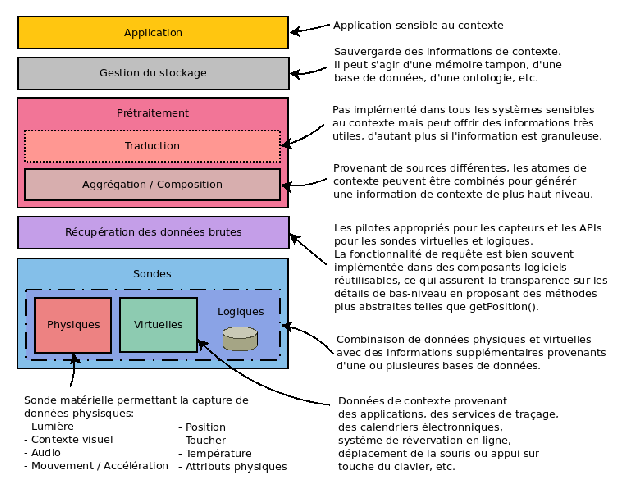
\includegraphics[width=.7\textwidth]{img/layered_conceptual_framework}
    \caption{Framework conceptuel d'un système sensible au contexte}
    \label{archi}
\end{figure}

\subsection{Sécurité et confidentialité}

{%\begin{figure}[H]
    \centering
    \begin{tabular}{l}
        La confidentialité est intrinsèquement liée au contrôle.
        \cite{ackerman_privacy_2001} \\
        %\em \footnotesize Mark Ackerman, Trevor Darrell, and Daniel Weitzner. 
        %Privacy in Context. \\
        %\em \footnotesize Human-Computer Interaction, 16(2):167–176, Décembre
        %2001. \\
    \end{tabular}
    %\caption{La confidentialité par Ackerman (2001)}
    %\label{fig:quote}
}%\end{figure}


Comme le contexte est susceptible de contenir des informations sensible sur des
personnes, leur situation géographique ou leur activité par exemple, il est
nécessaire de protéger le caractère personnel de ces données. Les systèmes
sensibles au contexte soulèvent des défis en termes de confidentialité
inhabituels et inconsidérés par les systèmes traditionnels. La question quant au
contrôle des différents capteurs et services n'est pas abordée dans Dey et al.
\cite{dey_conceptual_2001}, et bien souvent, des applications telles que le
Context Toolkit sont supposées être sous le contrôle d'un ''utilisateur''. Les
utilisateurs sont assignés comme propriétaires des données sondées par leurs
soins. Ils sont par ailleurs autorisés à octroyer l'accès à ces données à
d'autres utilisateurs.

Néanmoins, en ce qui concernent les sondes capables de déterminer la présence
d'individus dans une pièce ou à tout autre endroit, il n'existe aucunes
préconisations à ce sujet. C'est un point toutefois critique.

D'une manière générale, dans une environnement mettant à disposition un certain
éventail d'applications sensibles au contexte, un individu opère à travers de
multiples environnements sociaux, qui eux même font l'usage des données d'un
grand nombre d'autres individus.

Aspects souvent négligés, la sécurité et la confidentialité font partie des
composantes les plus importantes d'un système sensible au contexte, car la
protection des données sensibles doit être garantie.

\section{Systèmes et frameworks existants}

%\begin{wrapfigure}{r}{.4\textwidth}
\begin{figure}[H]
    \centerline{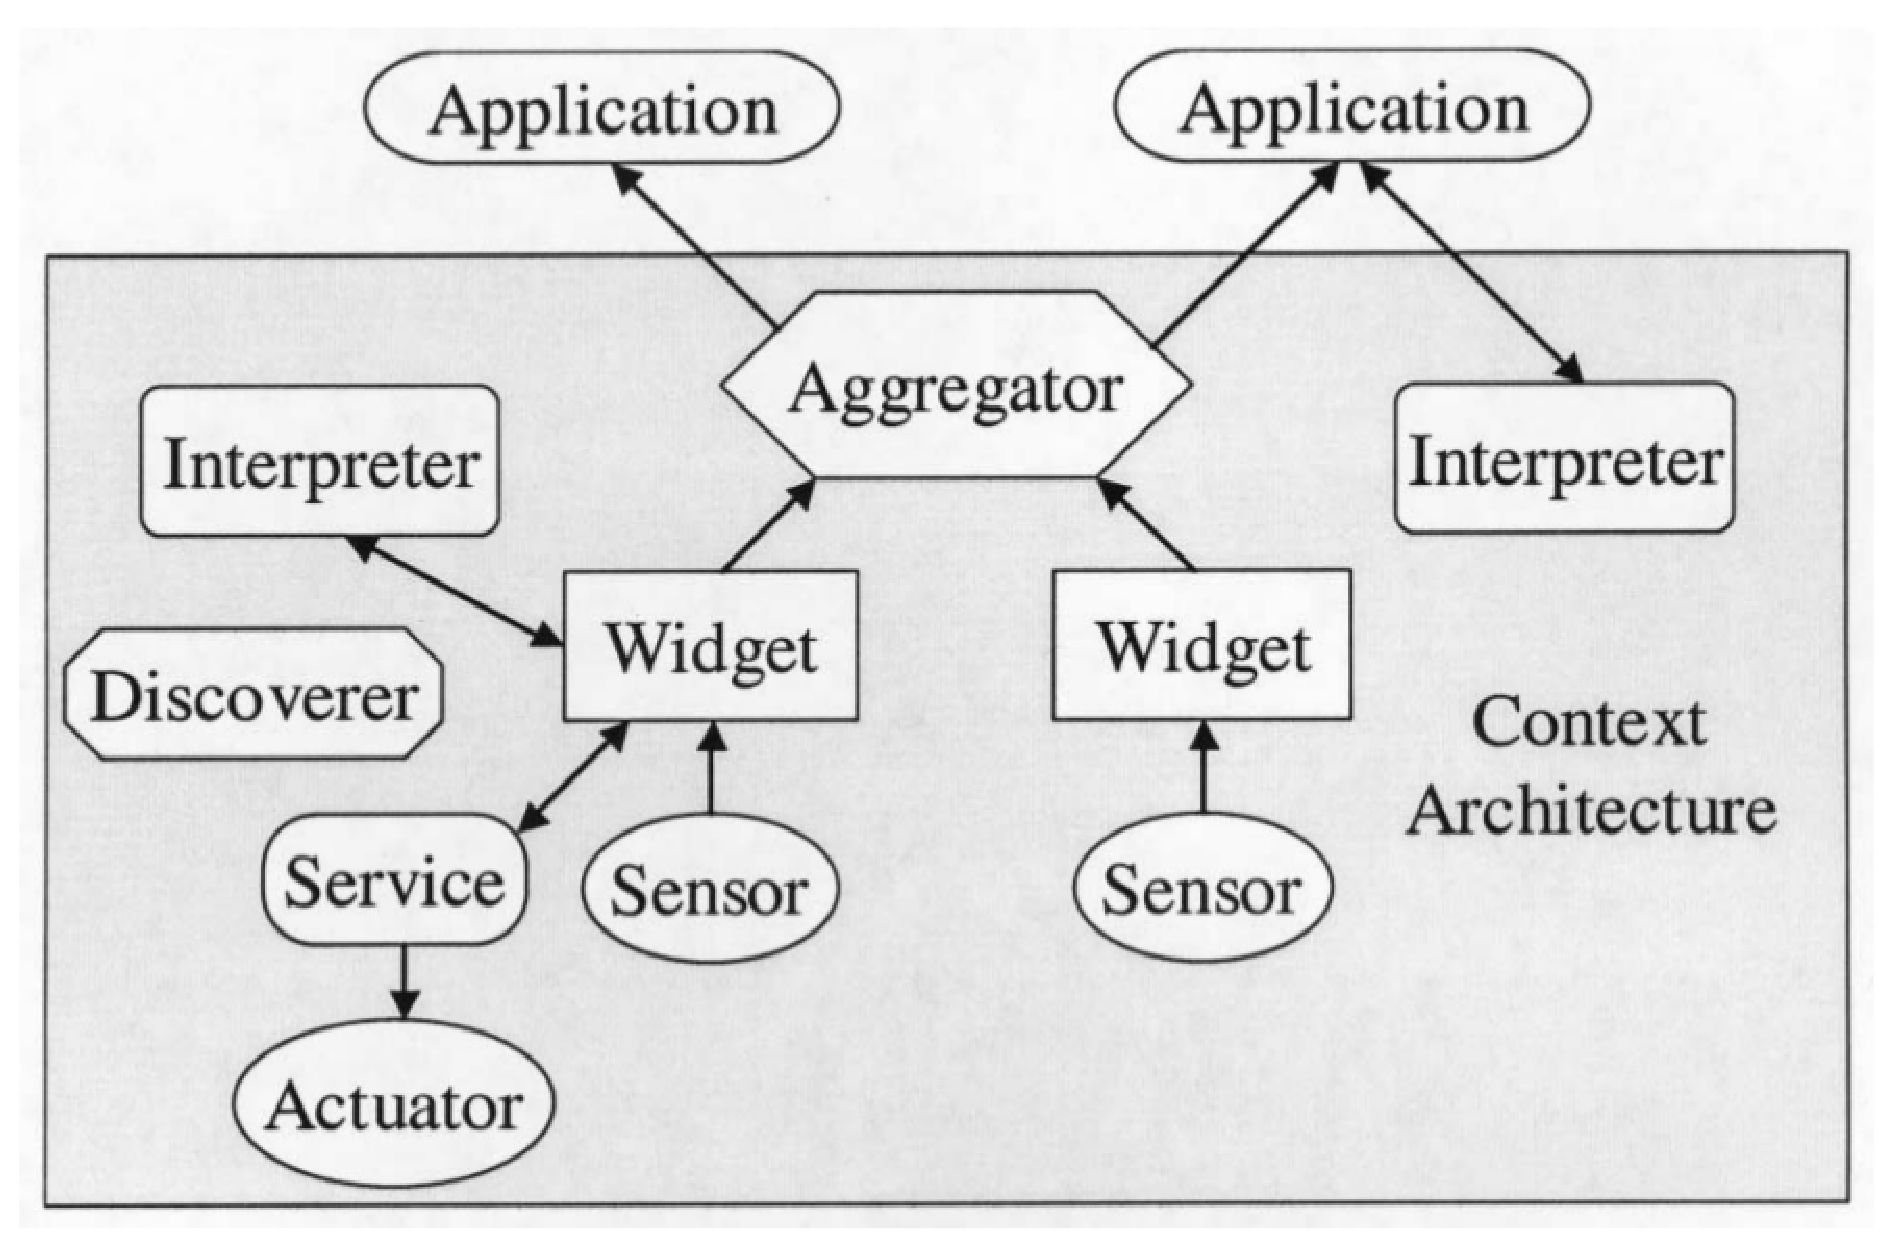
\includegraphics[width=.37\textwidth]{img/context_toolkit}}
    \caption{Exemple de configuration des composants du Context Toolkit}
    \label{Contexttoolkit}
%\end{wrapfigure}
\end{figure}

Le tableau \ref{ContextManagementFrameworkComparison} met en concurrence les
principaux aspects des approches existantes discutées précédemment. Le style
architectural d'un système sensible au contexte dépend en grande majorité de la
méthode d'acquisition des informations de contexte. Le principal critère
permettant de qualifier une approche architecturale comme raisonnable est la
démarquation claire entre l'acquisition de contexte et les composantes de
l'utilisateur proposée par Dey (2000) \cite{dey_providing_2000}. Tous les
frameworks présentés dans ce mémoire supportent cette scission des
préoccupations.

\begin{table*}%[h]
    \tiny
    \begin{tabularx}{\linewidth}{
      >{\raggedright\arraybackslash}X
      >{\raggedright\arraybackslash}X
      >{\raggedright\arraybackslash}X
      >{\raggedright\arraybackslash}X
      >{\raggedright\arraybackslash}X
      >{\raggedright\arraybackslash}X
      >{\raggedright\arraybackslash}X
      >{\raggedright\arraybackslash}X
    }
        \hline
        \textbf{Architecture} & 
        \textbf{Detection} & 
        \textbf{Modèle de contexte} &
        \textbf{Traitement du contexte} &
        \textbf{Découverte de ressources} &
        \textbf{Données de contexte historiques} &
        \textbf{Sécurité et confidentialité} & 
        \\
        \hline
        CASS &
        Intergiciel centralisé &
        Noeuds de capteurs &
        Modèle de données relationnel &
        Moteur d'inférence et base de connaissance &
        n.a. &
        Disponible &
        n.a.\\

        Cobra &
        Basée sur les agents &
        Modèle d'acquisition de contexte &
        Ontologies (OWL) &
        Moteur d'inférence et base de connaissance &
        n.a. &
        Disponible &
        Politiques en langage Rei\\

        Context Management Framework &
        Basée sur le "tableau noir" (blackboard) &
        Serveurs de ressources &
        Ontologies (RDF) &
        Service de reconnaissance de contexte &
        Serveurs de ressources et mécanisme de souscription &
        n.a &
        n.a.\\

        Context toolkit &
        Basée sur les widgets &
        Widgets de contexte &
        Tuples attribut/valeur &
        Interprétation et agrégation du contexte &
        Composant de découverte &
        Disponible &
        Propriété de contexte\\

        CORTEX &
        Modèle d'objet sensible &
        Framework de composants de contexte &
        Modèle de données relationnel &
        Framework de découverte de services &
        Framework de gestion des composantes ressources &
        Disponible &
        n.a.\\

        Gaia &
        MVC (étendu) &
        Fournisseurs de contexte &
        Prédicats quaternaires (DAML + OIL) &
        Module de contexte de service (logique de premier ordre) &
        Service de découverte &
        Disponible &
        Supporté (e.g., traçage sécurisé, confidentialité de localisation,
        contrôle d'accès)\\

        Hydrogen &
        Architecture trois couches &
        Adaptateurs variés pour les types de contexte &
        Orienté objet &
        Interprétations et agrégation des données brutes seulement &
        n.a. &
        n.a. &
        n.a.\\

        SOCAM &
        Distribué avec serveur central &
        Fournisseur de contexte &
        Ontologies (OWL) &
        Raisonneur contextuel &
        Service de localisation de service &
        Disponible &
        n.a.\\

        \hline
    \end{tabularx}
    \caption{Comparaison des framework existants pour la gestion du contexte}
    \label{ContextManagementFrameworkComparison}
\end{table*}

\subsection{Technologies de détection}

Dans chaque framework, la technologie de détection est implémentée différemment.
Afin de garantir la séparation détection/composants susmentionnée, il est
préférable d'encapsuler le mécanisme concret de détection dans des composantes
séparées. De plus, cela permet un accès aux données de contexte par le biais
d'interfaces définies. Il n'existe aujourd'hui aucun langage de description ou
d'ontologie permettant la réutilisation de l'information de contexte à travers
les différents intergiciels et frameworks. Par conséquent, des solutions
propriétaires ont vu le jour et sont utilisées par de nombreux frameworks.
Pour la détection d'information de contexte, SOCAM implémente l'approche la plus
sophistiquée : des services web fournissent de APIs (interfaces SOAP) pour les
sondes virtuelles externes et les sondes internes sont interrogées par
l'utilisation d'évènements contextuels. Ces évènements de contexte sont
modélisés en OWL et basés sur une ontologie prédéfinie.

\subsection{Représentations du contexte}

Afin d'obtenir des applications et services sensibles au contexte intelligents
et adaptables, le modèle et la logique de traitement du contexte pris en charge
individuellement par chaque framework est un critère majeur. Les ontologies
offrent un formalisme très riche pour représenter l'information de contexte.
Basé sur un modèle ontologique très sophistiqué, les raisonneurs peuvent dériver
de nouveaux concepts et ajuster le comportement d'un service en conséquence. La
représentation clé/valeur utilisée dans le Context Toolkit devient donc un
inconvénient majeur. Le fait que de tels attributs ne peuvent contenir aucune
sémantique restreint de manière considérable de le développement de procédés de
traitement et d'agrégation de contexte. De plus, les modèles non basés sur les
ontologies nécessitent un effort de programmation conséquent et couplent très
étroitement le modèle de contexte avec le reste du système. En outre, le
raisonnement et le partage de connaissances à travers les systèmes sont
impossibles en raison du manque de sémantique déclarative des programmes. SOCAM,
par exemple, fait l'usage d'une ontologie générale de haut niveau pour spécifier
des propriétés contextuelles de base communes et pour affiner cette même
ontologie. Dans le but de fournir des possibilités très granuleuses pour
spécifier et formaliser le contexte, certaines ontologies spécifiques à un
domaine peuvent être définies.

\subsection{Découverte de ressources}

Les mécanismes de découverte de nouvelles ressources sont très rarement
implémentés malgré l'importance d'un tel dynamisme, surtout dans un environnement
ubiquitaire, où les sources de contexte et les sondes disponibles changent
constamment. SOCAM est le seul système basé sur une architecture orientée
services. Il offre un service de localisation de services, qui se raccorde
dynamiquement aux fournisseurs de contexte disponibles. Cet fonctionnalité
manquante à la plupart des frameworks est en effet un tort puisque cela implique
que les sources de contexte utilisées doivent être stables et disponibles en
permanence, ce qui n'est pas toujours le cas dans les applications du monde
réel. Si une ou plusieurs sources de contexte se comportent mal, cela pourrait
conduire à une disponibilité réduite des services et des applications sensibles
au contexte.

\subsection{Gestion du contexte historique}

De la même manière, la majorité des frameworks conservent un historique des
données de contexte, mais aucun d'entre eux ne les exploitent vraiment.
Pourtant, cela pourrait permettre de fournir des services sensibles au contexte
fortement adaptables, si le contexte historique était utilisé pour implémenter
des algorithmes d'auto apprentissage. De plus, l'information de contexte
pourrait même être anticipée pour offrir proactivement un ensemble de services à
l'utilisateur.

\subsection{Sécurité et confidentialité}

Un autre aspect important à ne pas négliger est la sécurité et la
confidentialité. L'information de contexte le plus souvent considère le profil
utilisateur et d'autres informations sensibles. Pour cette raison, des concepts
sont requis pour exprimer des règles politiques et définir la propriété de
l'information de contexte. 

CoBrA inclus son propre langage de définition de politiques appelé Rei
\cite{kagal_policy_2005}, pour contrôler de manière flexible les accès aux
données de contexte. Ce langage de définition de politiques est calqué sur les
concepts déontiques de droits, d'interdictions, d'obligations et de dispenses,
et contrôle l'accès aux données grâce à des règles de politique modifiables
dynamiquement et dépendantes d'un domaine particulier. Gaia fait l'usage de
plusieurs mécanismes pour définir les restrictions en termes de confidentialité
et pour sécuriser les communications lors de localisations d'individus. Le
Contexte Toolkit implémente le concept de propriété des information de contexte,
qui autorise seulement le propriétaire des informations à consulter les données
sondées.

L'aspect sécurité n'est pas implémenté dans les autres frameworks. De nombreux
systèmes sont totalement dépourvus de modèles de sécurité, d'autres offrent des
mécanismes de sécurité très génériques et seulement quelques systèmes sont dotés
d'options de sécurités avancées et suffisantes.

\section{Conclusion}

Chacun des systèmes et frameworks présentés dans cet état de l'art implémentent
leur propre format pour la description des informations de contexte et des
mécanismes de communication dissemblables. La définition d'un modèle standard
d'abstraction des données de contexte semble être la priorité première dans
l'évolution des systèmes sensibles au contexte existants. Si le degré de
sophistication des systèmes distribués font leur force de calcul, leur
extrême complexité sont souvent la cause de leur boycott. Le modèle issu de
cette étude devra être simple, accessible, extensible et doté d'un haut degré de
formalisation.

% ex: set spelllang=fr spell: %
%%% Local Variables: ***
%%% mode: latex ***
%%% TeX-master: "thesis.tex" ***
%%% End: ***
